\documentclass{psta}% Подгружает макропакеты:
% \usepackage{inputenc,fontenc,babel,hyperref,url,xcolor,textcase,backref,enumitem,
%       amssymb,amscd,euscript,nameref,graphics,pdflscape,upref,rotating,array}
% Авторы могут использовать другие общедоступные макропакеты.
\usepackage{soulutf8}
\usepackage{fancyvrb}
\usepackage{attachfile2}
\usepackage{makecell}
\newcommand\thinhline{\Xhline{0.1pt}}
\newcommand\thinvline{\textcolor{lightgray}{\vrule width .2pt}}
%\usepackage{ragged2e}
%\tracingall
%\tracingnone
\newcommand{\diver}{\mathop{\mathrm{div}}\nolimits}

\selectlanguage{russian} % Не забывайте отметить возврат на русский язык
\newcommand\vitem[1][]{\SaveVerb[%
    aftersave={\item[\footnotesize\em{\UseVerb[#1]{vsave}}]}]{vsave}}
% Пожалуйста, уточните классификация Вашей статьи согласно УДК и MSC
\subjclass[UDC]{629.7.067.5}
\subjclass[2020]{97P99; 97U99}
% Выберите и укажите, пожалуйста, тип статьи и номер рубрики, см.\ ниже
%\ArticleType {RAR} % Research Article
\JournalRubric {0} % см. пояснение в тексте
%
\title [Шаблон стилевого файла]{Численное моделирование процесса обледенения в условиях крупных переохлажденных капель}
% \title [Сокращённое название для колонтитула]{Полный заголовок статьи}
\thanks{Работа поддержана грантом XXX №  YYY-ZZZ}

% Аналогично для каждого из остальных авторов
\author{Горячев, Алексей Владимирович}
\CRediT{1}{10.0\%}
\email{todo1@mail.ru}
\correspondent
\address{ФАУ Центральный институт авиационного моторостроения имени П.И. Баранова, Москва, Россия}
\info{info}
\orcid{0000-0000-0000-0000}
\image{pics/nobody}

\author{Горячев, Павел Алексеевич}
\CRediT{1}{10.0\%}
\email{todo2@mail.ru}
\correspondent
\address{ФАУ Центральный институт авиационного моторостроения имени П.И. Баранова, Москва, Россия}
\info{info}
\orcid{0000-0000-0000-0000}
\image{pics/nobody}

\author{Горячев, Д А}
\CRediT{1}{10.0\%}
\email{todo3@mail.ru}
\correspondent
\address{ФАУ Центральный институт авиационного моторостроения имени П.И. Баранова, Москва, Россия}
\info{info}
\orcid{0000-0000-0000-0000}
\image{pics/nobody}

\author{Нуриев, М В}
\CRediT{1}{10.0\%}
\email{todo4@mail.ru}
\correspondent
\address{ФАУ Центральный институт авиационного моторостроения имени П.И. Баранова, Москва, Россия}
\info{info}
\orcid{0000-0000-0000-0000}
\image{pics/nobody}

\author{Николаев, А А}
\CRediT{1}{10.0\%}
\email{todo5@mail.ru}
\correspondent
\address{ФАУ Центральный институт авиационного моторостроения имени П.И. Баранова, Москва, Россия}
\info{info}
\orcid{0000-0000-0000-0000}
\image{pics/nobody}

\author{Рыбаков, Алексей Анатольевич}
\CRediT{1}{10.0\%}
\email{rybakov_aan@nrcki.ru}
\correspondent
\address{\NRSCI}
\info{к.ф.-м.н., начальник отдела суперкомпьютерных технологий и систем Отделения суперкомпьютерны систем и параллельных вычислений НИЦ <<Курчатовский институт>>. Область научных интересов: суперкомпьютерное моделирование, комбинаторная оптимизация, параллельное программирование, функциональное программирование.}
\orcid{0000-0002-9755-8830}
\image{pics/rybakov}

\begin{abstract}
Предложен усовершенствованный метод, позволяющий повысить точность выполнения трехмерных расчетов процесса формирования льда на поверхностях летательного аппарата в атмосферных условиях крупных переохлаждённых капель (SLD).
Формирование ледяного нароста, описывается с использованием математических моделей течения жидких пленок SWIM, а также модели осаждения и разбрызгивания крупных капель при ударе о поверхность льда.
Предложено усовершенствование модели, позволяющее рассчитать процесс разбрызгивания как для сухих, так и для влажных поверхностей.
Валидация предложенного метода выполнена путём сравнения результатов расчётов с имеющимися экспериментальными данными, полученными на модельном профиле NACA0012 условиях SLD.
Данные расчётов показали лучшее соответствие с экспериментом по форме, размерам и локализации образующихся ледяных наростов по сравнению с результатами, полученными с использованием программного комплекса Ansys Fensap-Ice.
\end{abstract}

\keywords{обледенение, летательный аппарат, крупные переохлаждённые капли, метод конечных элементов, математическое моделирование.}

% Все метаданные должны также присутствовать на английском языке,
% заключённые в  \selectlanguage{english}...,\selectlanguage{russian}:
\selectlanguage{english}
\title[Template for submission]{Numerical modeling of the icing process under conditions of large supercooled droplets}
% \title [Short title for top colontitle]{The Full Engish Title}
% Last name, coma other names
\thanks{The work is supported by the grant XXX №  YYY-ZZZ}

\author{Goryachev, Alexey Vladimirovich}
\address{Central Institute of Aviation Motors, Moscow, Russia}
\info{info}
\email{todo1@mail.ru}
\orcid{0000-0000-0000-0000}

\author{Goryachev, Pavel Alexeevich}
\address{Central Institute of Aviation Motors, Moscow, Russia}
\info{info}
\email{todo2@mail.ru}
\orcid{0000-0000-0000-0000}

\author{Goryachev, D A}
\address{Central Institute of Aviation Motors, Moscow, Russia}
\info{info}
\email{todo3@mail.ru}
\orcid{0000-0000-0000-0000}

\author{Nuriev, M V}
\address{Central Institute of Aviation Motors, Moscow, Russia}
\info{info}
\email{todo4@mail.ru}
\orcid{0000-0000-0000-0000}

\author{Nikolaev, A A}
\address{Central Institute of Aviation Motors, Moscow, Russia}
\info{info}
\email{todo5@mail.ru}
\orcid{0000-0000-0000-0000}

\author{Rybakov, Alexey Anatolievich}
\address{\NRSCI}
\info{head of the Supercomputer Technologies and Systems Department of the Supercomputer Systems and Parallel Computing Division of the National Research Center "Kurchatov Institute". Research interests: supercomputer modeling, combinatorial optimization, parallel programming, functional programming.}
\email{rybakov_aan@nrcki.ru}
\orcid{0000-0002-9755-8830}

\begin{abstract}
An improved method is proposed that allows increasing the accuracy of three-dimensional calculations of the process of ice formation on aircraft surfaces under atmospheric conditions of large supercooled droplets (SLD).
Ice build-up formation is described using mathematical models of liquid film flow SWIM, as well as a model of deposition and splashing of large droplets upon impact with the ice surface.
An improvement of the model is proposed that allows calculating the splashing process for both dry and wet surfaces.
Validation of the proposed method is performed by comparing the calculation results with the available experimental data obtained on the NACA0012 model profile under SLD conditions.
The calculation data showed better agreement with the experiment in terms of shape, size and localization of the formed ice build-ups compared to the results obtained using the Ansys Fensap-Ice software package.
\end{abstract}

\keywords{icing, aircraft, large supercooled droplets, finite element method, mathematical modeling.}
\selectlanguage{russian} % Не забывайте отметить возврат на русский язык
%

\begin{document}
\Russian
\maketitle
% Если список авторов не умещается в колонтитул, используйте \shortauthors{...}

\section*{Введение}

Несущие аэродинамические поверхности летательных аппаратов и поверхности управления воздушным судном подвержены воздействию метеорологических условий обледенения, что может привести к недопустимому ухудшению аэродинамических характеристик ЛА.
Как правило, существующие системы защиты ЛА от воздействия условий обледенения рассчитаны на предотвращение опасного обледенения для облачных капель размером MVD = 20 мкм.

Однако, расследование катастрофы самолета ATR-72 близ Роузлоуна, штат Индиана, 31 октября 1994 года [1], вызванное потерей управления вследствие обледенения, пробудило повышенное внимание к метеорологическим исследованиям, подтвердившим существование в атмосферных облаках крупных переохлажденных капель (SLD) с размером MVD до 400 мкм.
Наросты льда, возникающие в условиях SLD могут привести к чрезвычайно серьезному ухудшению летно-технических характеристик самолета, включая: уменьшение угла сваливания, сопровождающееся увеличением скорости сваливания; снижение подъемной силы более чем на 60\% и увеличение лобового сопротивления до 200\%.
Указанные явления могут критическим образом влиять на безопасность полётов, поэтому при проектировании противообледенительных систем необходимо использовать расчётные методы для предотвращения недопустимого ухудшения аэродинамических характеристик элементов летательного аппарата [2].

Атмосферные облака SLD могут состоять как из переохлаждённой измороси <<freezing drizzle>>, так и из переохлаждённого дождя <<freezing rain>>.
Динамика этих капель имеет свои особенности [3].
Капли большого размера SLD двигаются по баллистическим траекториям, вследствие чего их выпадение на аэродинамические поверхности происходит ниже по течению от областей, защищенных противообледенительными системами, что приводит к потенциально неконтролируемому процессу образования льда на незащищённых поверхностях. Динамику крупных капель необходимо учитывать при вычислительном моделировании обледенения при проектировании систем противообледенительной защиты и в процессе сертификации авиационной техники.

Таким образом, при разработке мер противообледенительной защиты необходимо располагать расчётными инструментами, позволяющими оценивать эффективность защиты элементов авиационной техники от воздействия условий обледенения.
Для этого необходимо моделировать процессы движения подобных капель в несущем воздушном потоке, процесс их взаимодействия с поверхностью ЛА и процесс формирования льда.
Существующие программные комплексы, такие как ПК Ansys Fensap-Ice и ПК Flowvision [4, 5], обладают недостаточной точностью расчёта ледяных наростов сложных форм.
Кроме того, зарубежные ПК, такие как Ansys Fensap-Ice [4], требуют импортозамещения.
С целью устранения существующего пробела в процессе моделирования крупных переохлаждённых капель выполнено усовершенствование ПМ Кристалл [6] путём разработки математической модели обледенения в условиях SLD.

Решение поставленной задачи проводилось в следующих направлениях.

Во-первых, проблема течения капель в несущем потоке до их взаимодействия со стенкой.
Она включает в себя моделирование полей течений двухфазного дисперсного потока в постановке Эйлера и отработка методических проблем расчёта величин коэффициентов улавливания капель для спектра размеров SLD.
Данная проблема была решена путём использования ПМ Лазурит [7], что позволило рассчитывать поля течений двухфазного дисперсного потока в постановке Эйлера и определять величины коэффициентов улавливания капель для спектра размеров капель, характерных для SLD.

Во-вторых, проблемы взаимодействия крупных капель с твёрдыми поверхностями объекта и ледяного нароста.
Они включают в себя вопросы моделирования процесса формирования облака вторичных капель с учётом их термодинамического состояния, а также влияние этих капель на результирующий коэффициент улавливания и на процесс формирования льда.

\section{Метод расчета формирования льда в условиях крупных переохлажденных капель}

\subsection{Термодинамическая модель нарастания льда}

Описание термодинамических процессов обледенения в условиях SLD основывается на двух моделях Мессинжера [8] и течения жидких водяных плёнок SWIM (Shallow Water Icing Model) [9].
В работе [10] с использованием указанных моделей получена система дифференциальных уравнений переноса с источниковыми членами.
Уравнение сохранения массы
\begin{equation}
	\rho_w \left[ \frac{\partial h_w}{\partial t} + \diver(\overline{u} h_w) \right] = \dot{m}_{imp} - \dot{m}_{ice} - \dot{m}_{es} - \dot{m}_{film\_shed}
\end{equation}
представляет собой баланс массовых скоростей потоков воды в контрольном объёме на поверхности льда: $\rho_w \frac{\partial h_w}{\partial t}$ -- втекающих и вытекающих из контрольного объема, $\rho_w \diver(\overline{u} h_w)$ -- накапливающихся в контрольном объеме, $\dot{m}_{imp}$ -- выпадающих на поверхность капель, $\dot{m}_{ice}$ -- замерзающей воды, $\dot{m}_{es}$ -- покидающих контрольный объём в результате испарения или сублимации, $\dot{m}_{film\_shed}$ -- срывающихся с поверхности плёнки.
Аналогично уравнение сохранения энергии записывается в виде:
\begin{equation}
	\begin{aligned}
		\rho_w \frac{\partial h_w C_{p,w} \overline{T}}{\partial t} + \rho_w \diver(\overline{u} h_w C_{p,w} \overline{T}) = \\
		\dot{Q}_{kin} + \dot{Q}_{ice} - \dot{Q}_{imp} - \dot{Q}_{es} - \dot{Q}_{rad} - \dot{Q}_{conv} - \dot{Q}_{film\_shed} + \dot{Q}_{heat}
	\end{aligned}
\end{equation}

В уравнении (2) $\overline{T}$ -- температура поверхности льда.
Первый член в левой части уравнения (2) представляет собой изменение энтальпии воды, находящейся в контрольном объёме.
Второй член левой части выражает разность энтальпий втекающей и вытекающей воды.
Указанные тепловые потоки уравновешиваются в правой части уравнения суммой следующих потоков: $\dot{Q}_{ice}$ -- фазового перехода (замерзание воды/плавление льда) и охлаждения льда, $\dot{Q}_{kin}$ -- кинетической энергии выпадающих капель воды, $\dot{Q}_{imp}$ -- охлаждения выпадающих капель воды, $\dot{Q}_{es}$ -- испаряющейся/сублимирующейся воды, $\dot{Q}_{rad}$ -- излучения, $\dot{Q}_{conv}$ -- конвекции, $\dot{Q}_{film\_shed}$ -- охлаждения за счет срывающихся с поверхности пленки капель воды, $\dot{Q}_{heat}$ -- поток тепла на дне контрольного объема.

Массовая скорость потока капель, остающихся на поверхности после выпадения на неё, находится из уравнения
\begin{equation*}
	\dot{m}_{imp} = U_{\infty} \cdot LWC \cdot \beta_{drops} \cdot \left[ 1 - \frac{m_s}{m_0} \right]
\end{equation*}
где $LWC$ -- Liquid Water Content, концентрация воды в потоке воздуха; $U_{\infty}$ -- скорость потока, $\beta_{drops}$ -- коэффициент улавливания капель, $\frac{m_s}{m_0}$ -- коэффициента потери массы, $m_0$ -- масса капель, претерпевших соприкосновение с поверхностью, $m_s$ -- масса капель, претерпевших отскок или расплёскивание.

Использование коэффициента улавливания капель $\beta_{drops}$ позволяет рассчитать количество всех капель, претерпевающих столкновение с поверхностью льда.
При этом не учитываются эффекты образования вторичных капель.
При расчёте обледенения в условиях SLD нельзя пренебречь эффектами, связанными с отскоками и расплёскиванием капли в процессе её взаимодействия с поверхностью.
Последний член произведения в данном уравнении $1 - \frac{m_s}{m_0}$ позволяет учесть массовую долю капель, остающихся на поверхности после столкновения и не претерпевающих отскок или расплёскивание.
Для расчёта величины этого члена, характеризующего коэффициент потери массы, необходимо разработать соответствующие физические и математические модели.

\subsection{Физическая модель взаимодействия крупных капель с поверхностью}

В работе [11] выполнен качественный анализ влияния различных эффектов динамики крупных капель на процесс численного моделирования процесса обледенения.
Выполнена классификация этих эффектов на три категории (эффекты первого, второго и третьего порядка) на основе их влияния на процесс выпадения капель на стенку.
Эффекты первого порядка -- это взаимодействие капли со стенкой, которое возникает, когда капля, столкнувшаяся со стенкой, вся или частично отскакивает обратно в несущий поток.
Эффекты второго порядка включают распад капель, при этом капли подвергаются деформации под действием аэродинамических сил, распадаются на мелкие вторичные капли.
Другие физические эффекты динамики крупных капель, такие как гравитационные эффекты и эффекты турбулентности, считаются эффектами третьего порядка и пренебрежимо малы.
Исходя из результатов указанного анализа, при разработке модели обледенения в условиях SLD рассматриваются эффекты первого порядка: взаимодействие крупной капли со стенкой.

Варианты взаимодействия крупных капель SLD с поверхностью объекта представлены на рис. 1.: прилипание капли к поверхности рис. 1а, отскок рис. 1б, растекание по поверхности рис. 1в, разбрызгивание и частичное прилипание к сухой поверхности рис. 1г, разбрызгивание на смоченной поверхности рис. 1д.

\begin{figure}[ht]
\centering
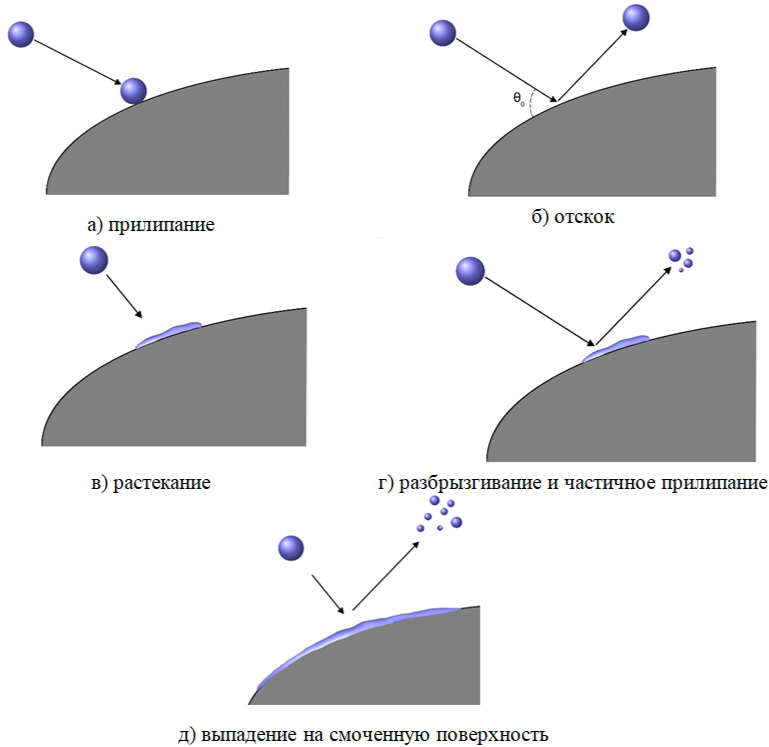
\includegraphics[width=0.7\textwidth]{pics/sld_with_surf_interact.png}
\caption{Варианты взаимодействия капли с поверхностью.}
\label{fig:sld_with_surf_interact}
\end{figure}

Из рассмотрения вариантов, представленных на рис. 1, следует, что не все выпадающие капли остаются на поверхности, поэтому следует уточнить величины коэффициентов улавливания путём корректного моделирования процесса их взаимодействия с поверхностью ледяного нароста. 

\subsection{Математическая модель взаимодействия крупных капель с поверхностью}

В соответствии с данными [12, 13] режимы, представленные на рис. 1 задаются числом Вебера для капли $We_d = \frac{\rho_{air} \cdot u_{n,0}^2 \cdot MWD}{\sigma}$, где $\overline{u}_d \overline{n}$ -- составляющая скорости капли, нормальная к поверхности профиля, $\sigma$ -- коэффициент поверхностного натяжения воды, $MWD$ -- средний медианный диаметр капли.

При $We_n \le 2$ -- реализуется прилипание капли к поверхности (рис. 1а) и ее дальнейшее участие в процессе льдообразования.
 
При $2 < We_n \le 10$ -- реализуется отскок капли (рис. 1б), происходит её участие в формировании вторичного потока частиц. Осаждение на поверхность отсутствует, результирующий коэффициента улавливания принимается нулевым.

Для расчёта скоростных характеристик капли, претерпевшей отскок, используются следующие соотношения:
\begin{equation*}
	f_{u,t} = \frac{u_{t,s}}{u_{t,0}} = \frac{5}{7}
\end{equation*}
\begin{equation*}
	f_{u,n} = \frac{u_{n,s}}{u_{n,0}} = -\left[ 0.9930 - 1.76 \cdot \theta_0 + 1.56 \cdot \theta_0^2 - 0.49 \cdot \theta_0^3 \right]
\end{equation*}
где $f_{u,n}$, $f_{u,t}$ -- отношение нормальной и тангенциальной составляющих скоростей, связанное с отскоком частицы от твердой поверхности, $u_{n,0}$, $u_{t,0}$ -- составляющие начальной скорости капли, нормальная и тангенциальная к поверхности, $u_{n,s}$, $u_{t,s}$ -- составляющие скорости капли после удара, нормальная и тангенциальная к поверхности, $\theta_0$ -- угол падения капли в радианах.

При $We_n > 10$ и $K_y \le K_{y,krit}$ -- реализуется растекание капли по поверхности (рис. 1в), то есть полное улавливание.
$K_y$ -- параметр разбрызгивания Ярина и Вейсса [14] вычисляется по формуле:
\begin{equation}
	K_y = \left[ \frac{3}{2} \cdot \left( \frac{LWC}{\rho_{air}} \right)^{\frac{3}{8}} \right] \cdot \left( Oh^{-\frac{2}{5}} W e_n \right)^{\frac{5}{16}}
\end{equation}
где $Oh = \frac{\mu_{air}}{\sqrt{\rho_{air} \cdot \sigma_d \cdot MWD}}$ -- критерий подобия Онезорге, $LWC$ -- водность потока, $\rho_{air}$ -- плотность воздуха, $Re_{d,n}$ -- число Рейнольдса, построенное на компоненте скорости капли, нормальной к поверхности профиля.

При $K_y > K_{y,krit}$ происходит разбрызгивание или частичное прилипание капли, которое может реализовываться как на сухой (рис. 1г), так и на влажной (рис. 1д) поверхности.

Варианты прилипание рис. 1а и растекание рис. 1в не представляют трудностей для расчёта, поскольку не требуют корректировки коэффициента улавливания.
Вариант отскока рис. 1б приводит к его обнулению коэффициента улавливания, но требует корректировки параметров отскочивших капель.
Наибольшую трудность представляют варианты рис. 1г, д, при которых происходит лишь частичное прилипание, а отскочившие капли образуют вторичный поток. 

При взаимодействии с сухой поверхностью (рис. 1г) расчёт количества, массы и скорости вторичных капель выполняется с использованием модели Трухильо [15].
Указанная модель применима при расчёте форм ледяных наростов в режиме <<rime ice>>.
Данный режим характеризуется полным замерзанием выпадающих капель и отсутствием плёнки жидкой воды на поверхности ледяного нароста.
Учет массы капель, разбрызгивающихся при ударе о поверхность аэродинамического профиля выполняется с применением коэффициента потери массы $\phi$, который рассчитывается по формулам (4).
\begin{equation}
	\begin{cases}
		& \phi(K_y) = \frac{3.8}{\sqrt{K_y}} \cdot \left( 1 - e^{-0.85 (K_y - K_{y,krit})} \right), K_y > K_{y,krit} = 17 \\
		& \phi(K_y) = 0, K_y \le K_{y,krit} = 17
	\end{cases}
\end{equation}
где параметр $K_y$ рассчитывается по формуле (3).

Количество вторичных капель может быть определено с использованием эмпирической модели Трухильо [15]:
\begin{equation}
	N = \frac{1}{22} \left( 0.0437 \cdot \left[ K \cdot \left( \frac{|\overline{u}_d|}{\overline{u}_d, \overline{n}} \right)^2 - K_{crit} \right] - 44.92 \right)
\end{equation}
где $K = Oh^{-\frac{2}{5}} \cdot We_n$ -- параметр Коассали, $K_{crit}$ -- критический параметр Коассали, который может быть рассчитан на основании уравнения (3), где $K_y \le K_{crit} = 17$.

Зная количество вторичных капель (5) и величину потери массы (4), диаметр вторичных капель может быть рассчитан из соотношения:
\begin{equation*}
	d_s = \left( \frac{\phi}{N} \right)^{\frac{1}{3}}
\end{equation*}

Средняя скорость вторичных капель $u_{d,s}$ также определяется с использованием эмпирической модели Трухильо [15] следующим образом:
\begin{equation}
	\frac{\overline{u}_{d,s} \cdot \overline{t}}{\overline{u}_d \cdot \overline{t}} = 0.85 + 0.0025 \arctan\left( \frac{\overline{u}_d \cdot \overline{t}}{\overline{u}_d \cdot \overline{n}} \right)
\end{equation}
\begin{equation}
	\frac{\overline{u}_{d,s} \cdot \overline{n}}{\overline{u}_d \cdot \overline{n}} = 0.12 + 0.002 \arctan\left( \frac{\overline{u}_d \cdot \overline{t}}{\overline{u}_d \cdot \overline{n}} \right)
\end{equation}

В уравнениях (6), (7) угол падения капли, от которого зависит вторичная скорость капель, представлен в виде нормальной и тангенциальной составляющей.

Кроме взаимодействия капель с твёрдой сухой стенкой, указанного на рис. 1г, на практике может реализовываться вариант рис. 1д.
Наличие на поверхности жидкой плёнки воды, как отмечается в работе [12], оказывает значительное влияние на процесс разбрызгивания.
Режим обледенения <<glaze ice>> наблюдается в условиях относительно высоких температур внешнего потока и характеризуется наличием жидкой плёнки воды на поверхности льда.
Причём, в зависимости от условий обледенения, плёнки воды могут иметь значительную толщину.
Наличие жидкости на поверхности может играть существенную роль, поскольку разбрызганные капли могут увлекать жидкость из пристеночной пленки [16], что наблюдалось экспериментально в работе [17].
При этом указывается, что масса разбрызганной моды может даже превосходить массу падающей капли. Для учёта эффектов, связанных с выпадением капель на влажные поверхности, использована модель Саменфинк [18].
В данной модели разбрызгивание наступает при величине параметра $S > 1$, который определяется формулой:
\begin{equation*}
	S = \frac{Re_d}{24 \cdot La_d^{0.419}}
\end{equation*}
где $La_d = \frac{\rho_d \cdot \sigma \cdot d_0}{\mu_d^2}$, $Re_d = \frac{u_{n,s} \cdot \sigma \cdot d_0}{v_d}$, $v_d$, $\mu_d$ -- статическая и динамическая вязкость жидкости, $u_{n,s}$ -- нормальная к поверхности составляющая скорости капли, $d_0$ -- диаметр капли до взаимодействия с поверхностью.

Характеристики вторичных капель определяются следующими формулами.

Диаметр вторичных капель $d_s$ по отношению к первичным $d_0$:
\begin{equation*}
	\frac{d_s}{d_0} = 1 - 0.03454 \cdot S^{0.175} \cdot \theta_0^{0.1239} \cdot La_d^{0.265}
\end{equation*}

Скорость вторичных капель $u_s$ по отношению к первичным $u_0$:
\begin{equation*}
	\frac{u_s}{u_0} = 0.08214 \cdot S^{-0.3384} \cdot \theta_0^{0.2936} \cdot \delta^{-03113} \cdot La_d^{0.1157}
\end{equation*}

Угол отскока капель:
\begin{equation*}
	\theta_s = 2.154 \cdot S^{1.0946} \cdot \theta_0^{0.03389} \cdot \delta^{-0.1589}
\end{equation*}

Нормальная $u_{n,s}$ и тангенциальная $u_{t,s}$ составляющие скоростей вторичных капель:
\begin{equation*}
	u_{n,s} = u_s \cdot \sin\left( \frac{\pi \cdot \theta_s}{180} \right)
\end{equation*}
\begin{equation*}
	u_{t,s} = u_s \cdot \cos\left( \frac{\pi \cdot \theta_s}{180} \right)
\end{equation*}

Коэффициент потери массы рассчитывается по формуле:
\begin{equation*}
	f_{m_{Sp}} = \frac{m_s}{m_0} = 0.0866 \cdot (S - 1)^{0.3188} \cdot \theta_0^{0.1223} \cdot \delta^{-0.9585}
\end{equation*}

Количество образовавшихся вторичных капель рассчитывается по формуле (5).

Анализ моделей разбрызгивания, представленный в работе [11], показывает, что обе модели Трухильо [15] и Саменфинк [18] показывают хорошие результаты при валидации с экспериментальными данными в диапазоне скоростей до 78 м/c.
В соответствии с выводами данной работы предпочтение было отдано модели Трухильо на том основании, что данная модель демонстрирует примерно аналогичные результаты по разбрызгиванию для капель с размером MVD=92 мкм и MVD=236 мкм и результаты могут быть экстраполированы за пределы экспериментальных данных (на диапазон повышенных скоростей).
При этом отмечено, что модель Саменфинк при указанном выше увеличении размеров капель демонстрирует более высокие величины потери массы, что по мнению авторов [11] не представляется реалистичным.
Для преодоления указанных недостатков в данной работе предлагается объединение обоих моделей с использованием формулы:
\begin{equation}
	\frac{m_s}{m_0} = min(f_{m_{Sp}}, \phi(K_y))
\end{equation}

Графически данное объединение двух моделей представлено на Рис. 2.

\begin{figure}[ht]
\centering
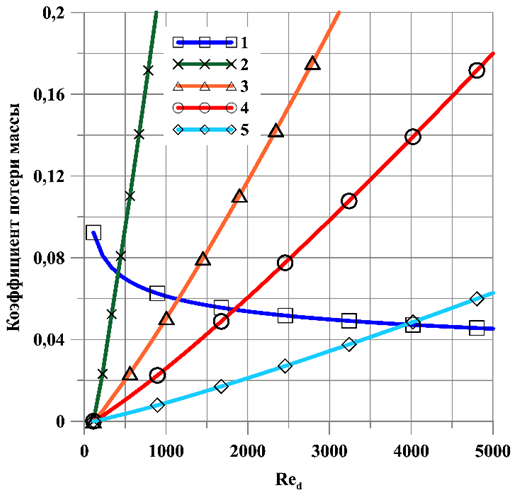
\includegraphics[width=0.5\textwidth]{pics/chart2.png}
\caption{Коэффициент потери массы, рассчитанный по различным моделям: 1 –Трухильо, 2 – Саменфинк, высота плёнки 10 мкм, 3 –Саменфинк, высота плёнки 50 мкм, 4 –Саменфинк, высота плёнки 100 мкм, 5 –Саменфинк, высота плёнки 300 мкм.}
\label{fig:chart2}
\end{figure}

\subsection{Метод расчета с использованием предложенной модели}

При решении уравнений (1)-(2) используется поверхностная неструктурированная расчетная сетка с треугольными ячейками, пример которой приведен на рис. 3.
Физические параметры привязаны к центрам ячеек.

\begin{figure}[ht]
\centering
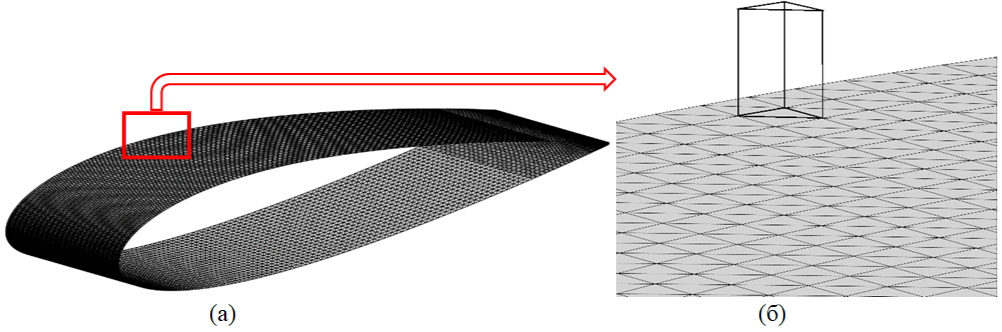
\includegraphics[width=1.0\textwidth]{pics/surf_mesh.png}
\caption{Пример поверхностной неструктурированной расчетной сетки.}
\label{fig:surf_mesh}
\end{figure}

Пример сетки, построенной на поверхности ледяного нароста, сформировавшегося на элементе сложной формы, показан на рис. 3а.
Количество ячеек 27 926. На рис. 3б детально показан фрагмент сетки с контрольным объемом над одной из расчетных ячеек.

Каждая итерация вычислений состоит из двух основных фаз: расчет протекания потоков массы и тепла между смежными ячейками через ребра расчетной сетки (моделирование течения пленки по поверхности) и определение состояния ячеек сетки (вычисление физических величин внутри ячеек).
Для расчета течения жидкой пленки по поверхности используется конечно-объемный метод с противопотоковой схемой Роу первого порядка [19, 20]. 
Для определения состояния ячейки на каждой итерации расчетов решается система уравнений относительно переменных $\dot{m}_{ice\_surf}$, $T_{surf}$, $h_w$, составленная из уравнения массового баланса и уравнения теплового баланса.
В зависимости от фазового состояния льда/воды в ячейке эту систему уравнений можно замкнуть, уменьшив количество переменных до двух [21].

Если в ячейке температура поверхности $T_{surf} = 0^{\circ}С$ и на поверхности присутствуют лёд и вода, то рассматривается состояние глазурного льда (GLAZE\_ICE).
В этом случае задача сводится к решению системы их двух линейных  уравнений относительно $h_w$ и $\dot{m}_{ice\_surf}$.
Если температура поверхности отрицательная $T_{surf} < 0^{\circ}С$ и плёнка воды отсутствует $h_w = 0$, то рассматривается состояние изморози (RIME\_ICE).
Если температура поверхности положительна $T_{surf} > 0^{\circ}С$ и слой льда отсутствует льда $\dot{m}_{ice\_surf} = 0$, то рассматривается состояние жидкой пленки (WET\_SURFACE).
Если в ячейке отсутствует и лед, и вода, то рассматривается состояние сухой поверхности (DRY\_SURFACE).
Для состояний RIME\_ICE, WET\_SURFACE, DRY\_SURFACE система уравнений сводится к одному нелинейному уравнению относительно температуры поверхности $T_{surf}$. 
Состояние ячейки считается определенным корректно, если выполнены условия совместности:
\begin{equation*}
	\begin{cases}
		& h_w \ge 0 \\
		& \dot{m}_{ice} \ge 0 \\
		& h_w \overline{T} \ge 0 \\
		& \dot{m}_{ice} \overline{T} \le 0
	\end{cases}
\end{equation*}

Если при определении физических величин для какого-либо состояния ячейки условия совместимости нарушаются, то предпринимается попытка найти решение с использованием другого состояния, как это показано на рис. 4.
Например, при неудачном решении для состояния GLAZE\_ICE сначала предпринимается попытка поиска решения для состояния RIME\_ICE, а затем для состояния WET\_SURFACE. Если решение не может быть найдено ни для какого состояния, то фиксируется аварийная ситуация.

\begin{figure}[ht]
\centering
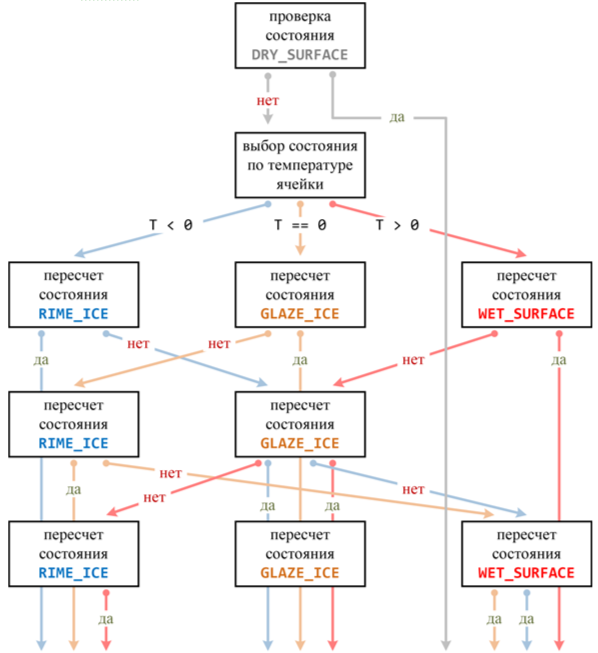
\includegraphics[width=0.7\textwidth]{pics/scheme.png}
\caption{Последовательность поиска решения для разных состояний ячейки.}
\label{fig:scheme}
\end{figure}

\subsection{Особенности реализации ПМ Кристалл}

Наиболее затратной по времени процедурой в процессе расчетов ПМ Кристалл является решение нелинейного уравнения с одной переменной.
В процессе проведения расчетов формула этого уравнения не может быть записана явно, а некоторые члены уравнения не являются дифференцируемыми. Поэтому для решения использовался комбинированный метод, основанный на методе хорд с использованием отдельных итераций метода бисекций для предотвращения зацикливания [22].

Для ускорения вычислений используется двухуровневое распараллеливание MPI+OpenMP. При распараллеливании вычислений по MPI декомпозиция расчетной сетки выполняется с помощью алгоритма Фархата, либо с помощью алгоритма пузырькового роста, начиная со случайных опорных ячеек [23].
Для улучшения масштабируемости используется механизм сокрытия издержек на межпроцессные обмены за основными вычислениями.
Для этого ячейки каждого домена разбиваются на два подмножества: граничные ячейки -- граничащие с границей домена, и внутренние ячейки -- все остальные ячейки.
На каждой итерации расчетов сначала обрабатываются граничные ячейки всех доменов, а затем межпроцессные обмены запускаются одновременно с обработкой внутренних ячеек доменов, как это показано на рис. 5.

\begin{figure}[ht]
\centering
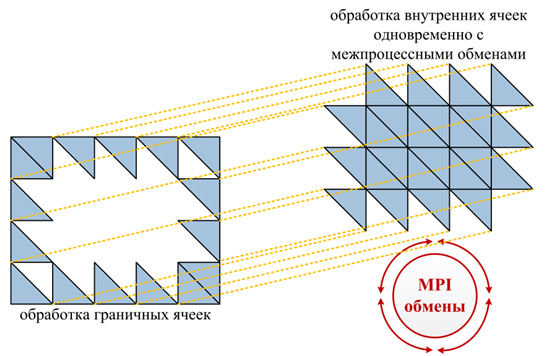
\includegraphics[width=0.7\textwidth]{pics/mpi.png}
\caption{Организация межпроцессных обменов между доменами расчетной сетки.}
\label{fig:mpi}
\end{figure}

При проведении одной итерации расчетов производится два основных цикла вычислений: цикл по всем ребрам расчетной сетки для пересчета протекания массового и теплового потоков и цикл всем ячейкам сетки для определения их состояний.
При обработке ребра расчетной ячейки выполняется изменение консервативных величин инцидентных ему ячеек.
Для устранения конфликтов по данным, потенциально возникающих при параллельной обработке ребер, множество ребер разбивается на множества неконфликтующих ребер путем построения реберной раскраски дуального графа сетки.

После расчета высоты ледяных наростов в каждой ячейке выполняется перестроение расчетной сетки с учетом накопленного льда.
В ПМ Кристалл используется набор различных методов перестроения расчетной сетки [24], в том числе методы перестроения с представлением объема льда в ячейке с помощью треугольных призм и усеченных пирамид, многоуровневое итерационное перестроение поверхности, перестроение с сохранением объема льда в ячейках [25].

\section{Результаты расчетов формирования льда в условиях крупных переохлажденных капель}

Расчёт форм льда выполнялся программным комплексом ПМ Кристалл [6] с использованием предлагаемой модели. Результаты представлены на рис. 6 в сравнении с ПК Ansys Fensap-Ice и с данными испытаний.
Предлагаемая модель позволяет повысить точность трехмерных расчетов процесса обледенения и получить ледяной нарост, более соответствующий экспериментальным формам.

\begin{figure}[ht]
\centering
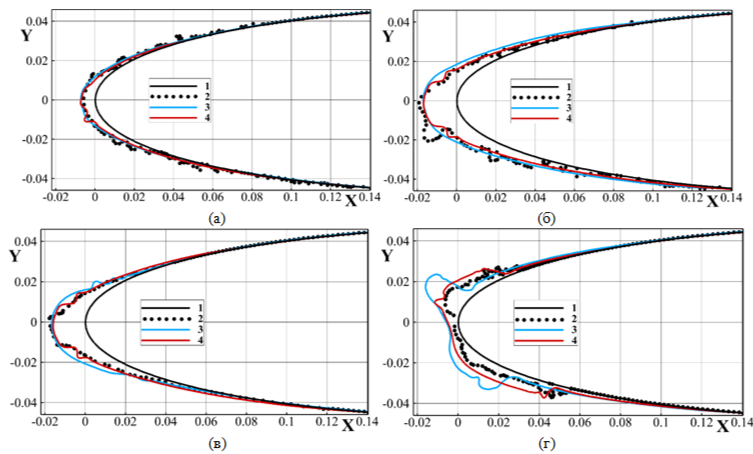
\includegraphics[width=1.0\textwidth]{pics/chart6.png}
\caption{Формы льда на режимах табл. 1, полученные с использованием различных программных комплексов, в сравнении с экспериментальными данными: (а) -- режим №1 табл. 1, (б) -- режим №2 табл. 1, (в) -- режим №3 табл. 1, (г) -- режим №4 табл. 1; 1 -- профиль NACA0012, 2 -- эксперимент [26], 3 -- ПМ Ansys Fensap-Ice [4], 4 -- настоящая модель.}
\label{fig:chart6}
\end{figure}

\begin{table}\footnotesize
\caption{Условия моделирования обледенения в условиях крупных переохлаждённых капель SLD.}
\begin{tabular}{|c|c|c|c|c|c|c|m{40mm}|}
\hline
N & LWC & MVD & OAT & Высота & Скорость & Угол атаки & Продолжительность воздействия условий обледенения \\ 
\hline
1 & 0.3 & 104 & -10 & 0 & 65 & 2 & 450 \\
2 & 0.3 & 180 & -25 & 0 & 158 & 2 & 450 \\
3 & 0.3 & 40 & -25 & 0 & 158 & 2 & 450 \\
4 & 0.3 & 104 & -10 & 0 & 163 & 2 & 450 \\
\hline
\end{tabular}
\end{table}

На рис. 6 представлено сравнение результатов расчета по предлагаемой модели с ПК Ansys Fensap-Ice [4] и с экспериментальными данными [26], выполненными в условиях крупных переохлаждённых капель SLD.

В результате расчёта форм льда на режимах 1, 2 и 3 получено хорошее соответствие экспериментальным данным по границам областей обледенения и толщинам льда в лобовой части ледяного нароста рис. 6а, 6б, 6в.
В расчётах получена более гладкие формы льда по сравнению с экспериментом, в котором наблюдалось образование крупных ледяных сталактитов, направленных навстречу потоку.
Подобные формы образуются в процессе течения жидкости по поверхности льда, её частичного срыва во внешний поток в виде капель и вторичного выпадения этих капель на поверхность.
Однако, подобные явления протекать не могут, поскольку на указанных режимах реализуются условия обледенения типа «rime ice», при этом величина температуры на поверхности льда ниже $0^{\circ}С$ и отсутствует течение жидкой воды.
 
Указанное несоответствие можно объяснить недостаточным переохлаждением крупных капель, получаемых при испытаниях, поскольку их генерация в условиях стенда является крайне сложной задачей.
Недоохлаждённые крупные капли при выпадении на поверхность льда могут растекаться в виде жидкой плёнки, образуя поверхность с ледяными сталактитами, наблюдавшимися в испытаниях.
В наибольшей степени данное явление наблюдается для наиболее крупных капель, которые труднее всего поддаются переохлаждению.
Максимальное образование сталактитов наблюдалось на режимах 1 и 2, рис. 6а, 6б, для которых величина MVD составляла 104 и 180 мкм, соответственно.
На режиме 3, рис. 6в, для которого величина MVD=40 мкм, образование сталактитов существенно меньше. 

В результате расчёта на режиме 3 была получена форма ледяного нароста с характерным массивным выступом в области передней критической точки рис. 6в. образование подобной формы, вероятно, объясняется зависимостью величины разбрызгивания крупных капель от угла их падения на поверхность льда.
Предложенная модель позволяет достаточно точно рассчитать подобную форму.

Аналогичное явление наблюдается и на режиме 2, рис. 6б. В расчёте, аналогично с режимом 3, получена форма массивного выступа, однако в испытаниях передний выступ значительно опущен вниз с образование рога в нижней части. Данное явление объясняется недостаточным переохлаждением крупных капель вследствие которого часть жидкости под воздействием воздушного потока и силы тяжести стекает вниз.
При этом весь массивный выступ, образующийся в расчёте при полном замерзании капель, в эксперименте как бы “стекает” вниз.
 
Для образования массивного выступа рис. 6б, 6в необходимо достаточное количество воды, которое обеспечивается на режимах 2 и 3 высокой скоростью потока 158 м/с. На режиме 1 рис. 6а подобный выступ не успевает сформироваться вследствие недостаточного количества воды, поступающей из потока со скоростью 65 м/с.

Таким образом, с учётом указанных соображений, расчётные формы льда, полученные на режимах 1, 2 и 3 с использованием предложенной модели, хорошо соответствуют экспериментальным данным. 

Как и формы, полученные с использование предлагаемой методики, формы льда, рассчитанные с использованием ПМ Ansys Fensap-Ice [4], являются гладкими, с отсутствием крупных сталактитов рис. 6а, 6б, 6в. Однако, в расчётах ПМ Ansys Fensap-Ice не наблюдается появление массивного выступа в районе лобовой части ледяного нароста.

Наиболее сложным случаем моделирования представляется режим 4 рис. 6г на котором реализуются условия обледенения типа «glaze ice», при этом величина температуры на поверхности льда равна 0°С и присутствует течение жидкой воды. Расчёт с использованием предлагаемой модели даёт довольно точное предсказание толщины льда в передней критической точке, а также в периферийных областях ледяного нароста. Расчёт формы льда, выполненный ПМ Ansys Fensap-Ice, имеет большую толщину льда и более рогообразную форму по сравнению с результатами по предлагаемой методике. 

Таким образом, представленные результаты расчёта имеют хорошее совпадение с экспериментальными данными и показывают преимущества применения модели в сравнении с другими современными программными комплексами. Предлагаемая модель позволяет выполнять расчёт процесса обледенения элементов авиационной техники в широком диапазоне условий обледенения, включая условия жидких переохлаждённых капель.

\section*{Заключение}

Для описания нестационарного процесса формирования льда на поверхностях летательного аппарата в атмосферных условиях крупных переохлаждённых капель (SLD) предложен метод, позволяющий повысить точность расчета форм, локализации ледяных наростов и температурного состояния обледеневающей поверхности. 

Формирование ледяного нароста, описывается с использованием следующих математических моделей: течения жидких пленок на поверхности льда SWIM, а также модели осаждения и разбрызгивания крупных капель при ударе о поверхность льда. Предложено усовершенствование модели, позволяющее рассчитать процесс разбрызгивания как для сухих, так и для влажных поверхностей. Валидация предложенного метода выполнена путём сравнения результатов расчётов с имеющимися экспериментальными данными, полученными на модельном профиле NACA0012 условиях SLD. Данные расчётов показали лучшее соответствие с экспериментом по форме, размерам и локализации образующихся ледяных наростов по сравнению с результатами, полученными с использованием программного комплекса Ansys Fensap-Ice.

\section*{Список литературы}

\begin{enumerate}
\item Pereira CM Status of NTSB aircraft icing certification related safety recommendations issued as a result of the 1994 ATR-72 accident at Roseland // AIAA meeting paper, January 1997.
\item Горячев П.А., Бурцев С.А. Влияние обледенения на аэродинамические характеристики элементов авиационной техники при полетах в условиях ледяных кристаллов и смеси фаз. Двигателестроение, 2025, № 1 (299), с. 44.
\item Tan SC, Papadakis M General efects of large droplet dynamics on ice accretion modeling // AIAA 2003-392, January 2003.
\item Программный комплекс Ansys FENSAP-ICE: Ice Accretion Simulation Software // 2019. https://www.ansys.com/products/fluids/ansys-fensap-ice.
\item Программный комплекс FlowVision компании ООО «ТЕСИС» // 2020. https://flowvision.ru/ru/.
\item Программный модуль компьютерного моделирования процесса обледенения элементов авиационных силовых установок («КРИСТАЛЛ 2023»). Авторы: Горячев А.В., Горячев П.А., Рыбаков А.А. // Свидетельство о государственной регистрации программы для ЭВМ № 2023666962. Дата регистрации: 08.08.2023.
\item Программный модуль компьютерного моделирования на основе уравнений RANS/URANS («Лазурит-RАNS») // Свидетельство о государственной регистрации программы для ЭВМ № 2019661604. Дата регистрации: 04.09.2019.
\item Messinger B.L. Equilibrium temperature of an unheated icing surface as a function of airspeed // J. of the Aeronautical Sciences. 1953. V. 20. № 1. P. 29.
\item Bourgault Y., Beaugendre H., Habashi W. G. Development of a shallow-water icing model in FENSAP-ICE // J. of Aircraft. 2000. V. 37. № 4. P. 640.
\item Бендерский Л. А., Горячев А. В., Горячев П. А., Горячев Д. А., Любимов Д. А., Студенников Е. С. Особенности моделирования тепломассообменных процессов при формировании льда в условиях атмосферного облака, состоящего из переохлаждённых капель // ТВТ. 2024. Т. 62. № 2. С. 222.
\item Wright W.B., Potapczuk M.G. Semi-Empirical Modeling of SLD Physics // 42nd Aerospace Sciences Meeting and Exhibit, Reno, Nevada, January 5–8, 2004. NASA/TM—2004-212916.
\item Bai C., Gosman A. Development of Methodology for Spray Impingement Simulation // SAE Technical Paper, 1995.
\item L.P. Raj, J. Lee, R.S. Myong, Ice accretion and aerodynamic effects on a multielement airfoil under SLD icing conditions // Aerosp. Sci. Technol. No 85,  pp 320–333, 2019.
\item Yarin A. L and Weiss D. A. Impact of drops on solid surfaces: self-similar capilary waves, and splashing as a new type of kinematic discontinuity // Journal of Fluid Mechanics, Vol. 283, pp 141–173, January 1995.
\item Trujillo M. F, Mathews W. S, Lee C. F, and Peters J. F. Modelling and experiment of impingement and atomization of a liquid spray on a wall // International Journal of Engine Research, Vol. 1, No 1, pp 87–105, 2000.
\item Bai C., Gosman A. D. Development of Methodology for Spray Impingement Simulation // International Congress and Exposition Detroit, Michigan February 27-March 2, 1995.
\item Mutchler, C. K. The size, travel and composition of droplets formed by waterdrop splash on thin water layers // Ph.D Thesis, University of Minnuesota, 1970.
\item Samenfink, W., Elsaber, A., Dullenkopf, K., and Wittig, S. Droplet interaction with Shear-Driven Liquid Films: Analysis of Deposition and Secondary Droplet Characteristics // Int. J. of Heat and Fluid Flow, v. 20, pp. 462–9, 1999.
\item Phongthanapanich A. A stable hybrid Roe scheme on triangular grids // International Journal for Numerical Methods in Fluids, 2020, 1-23, https://doi.org/10.1002/fld.4916
\item Elong A., Zhou L., Karney B., Xue Z., Lu Y. A comprehensive numerical overview of the performance of Godunov solutions using Roe and Rusanov schemes applied to dam-break flow // Water, 2024, 16, 950, https://doi.org/10.3390/w16070950
\item Горячев П. А., Бурцев С.А. Математическая модель формирования льда в условиях наличия ледяных кристаллов и смеси фаз // ТВТ. 2025. Т. 63. № 1. С. 50.
\item Mohammadi N., Mehdipour-Ataei S., Mohammadi M. Numerical methods for solving nonlinear equations // in Mahdavi Tabatabaei N., Bizon N. (eds) Numerical Methods for Energy Applications, 2021, Power Systems, Springer, https://10.1007/978-3-030-62191-9\_5
\item Головченко Е. Обзор алгоритмов декомпозиции графов // Препринты ИПМ им. М.В.Келдыша, 2020, 2, 38, https://doi.org/10.20948/prepr-2020-2
\item Meshcheryakov A., Rybakov A. Evolution of the surface computational mesh in the ice accretion process // Lobachevskii Journal of Mathematics, 2023, 44, 11, 361-378, https://doi.org/10.1134/S1995080223110367
\item Tong X., Thompson D., Arnoldus Q., Collins E., Luke E. Three-dimensional surface evolution and mesh deformation for aircraft icing applications // Journal of Aircraft, 2016, 54, 1047-1063, https://doi.org/10.2514/1.C033949
\item Reinhard Puffing. Ice Genesis Icing Database // 2021. https://icing-database.eu/index.php.
\end{enumerate}











\section{Назначение макропакета и подготовка к его использованию}\label{sec:general}
Макропакет доступен \Href{http://psta.psiras.ru/publ-conditions/psta.zip}{по ссылке}, создан для обработки современным \texttt{pdflatex}, но допускает и другие способы обработки LaTeX.

\subsection{Подготовка к работе}
Ожидается, что авторы знакомы с общепринятыми требованиями
\begin{itemize}
\item к структуре и содержанию научных публикаций \cites{Safonov2007,Fradkov2003,Sviderskaya2011,KirillovaLong,KirillovaShort},
\item к набору в \LaTeX\ \cites{Stolarov,Vorontsov,Syutkin},
\item к оформлению сложных формул в  AMS\LaTeX\ \cites{AMSshort,Mathmode}.
\end{itemize}

Для улучшения качества pdf и получения возможности доводки корректуры полезно установить пакет \verb|cm-super|.

Перед началом работы рекомендуется раскрыть с~поддиректориями архив psta.zip %\attachfile{psta.zip}
и обработать файл \textsf{mail-ru.tex} в Вашей системе. К сожалению, LaTeX быстро меняется, и, например, базовая установка Миктех, если не включать обновления, застревает на символе номера.
Если компиляция \textsf{main-ru.pdf} прошла успешно, то можно поменять в \textsf{main-ru.tex} заполнение титульной информации, а затем и содержимое.



\subsection{Опции макропакета}
Несколько опций могут использоваться в первой строке исходного файла \verb|\documentclass[|...\verb|]{psta}| в квадратных скобках:
\begin{description}
% Команда \vitem из пакета fancyvrb заменяет неработающее сочетание \item \verb
\vitem |russain|, \verb |english| настраивают оформление для статей на русском языке или на английском языке;
\vitem |blind| для отправки PDF рецензенту аккуратно прячет персональную информацию. Если в тексте статьи есть фрагменты, которые могут идентифицировать автора, то автор прячет их в аргумент команды \verb|\HideFromPeer{|...\verb|}|, чтобы избежать лишнего редактирования;
\vitem |secsymbol| добавляет символ параграфа в заголовки, при этом  гиперссылка \verb|\ref{|метка\footnote{русские буквы в метках пока не работают.}\verb|}| на (под)раздел  \verb|\label{|метка\verb|}| приобретает желаемый вид как в \Href{http://psta.psiras.ru/read/psta2018_1_53-83.pdf\#page=7}{этой опубликованной статье}.
\vitem |sloppy| заставляет команду \verb|\sloppy| делать пробелы между словами и формулами более растяжимыми только до конца текущего абзаца.
\end{description}

\section{Титульная информация о статье}\label{sec:meta}
Преамбула исходного файла (до \verb|\begin|\verb|{document}|) должна содержать всю титульную информацию, включая информацию об авторах на русском и английском языках.
Язык переключает команда  \verb|\selectlanguage|\verb|{|...\verb|}|.

\subsection{Тип и рубрика статьи}

Отличный от RAR тип статьи указывается командой \verb|\ArticleType{|...\verb|}| с аргументом из \Altref{таблицы}{tab:ArticleType},
\begin{table}\footnotesize
\caption{Типы статей}\label{tab:ArticleType}
\begin{tabular}{|c|m{30mm}<{\raggedright}!{\thinvline}m{61mm}|}
\hline
Аргумент&\hfil\hfil Значение	 &\hfil Пояснение\\
\hline
PER	& Персоналия		 (Personal)& От редакционной коллегии.\\\thinhline
RAR	& Научная статья 	 (Research Article)& Текст статьи должен ясно описывать, обосновывать и обсуждать значимо новые уникальные результаты и не содержать 
повторений, ненужных для понимания результатов, их новизны и значимости. 
Численная оценка заимствований не значима.\\\thinhline
REV	& Обзорная статья	 (Review Article)&Обзор, по-новому представляющий состояние исследований в области и выявляющий ключевые направления дальнейшего развития.\\\thinhline
SCO	& Краткое сообщение 	 (Short~Communication)& По особому решению редакционной коллегии. \\
\hline
\end{tabular}
\end{table}
(как в метаданных \Href{https://www.elibrary.ru/}{E-library}).

Номер рубрики \verb|\JournalRubric{|...\verb|}| авторы выбирают на основании \Altref{таблицы}{tab:JournalRubric}, в которой зачёркнуты прежние названия рубрик.
\begin{table}\footnotesize\renewcommand{\arraystretch}{1.3}
\caption{Рубрики журнала и научные специальности}\label{tab:JournalRubric}
\begin{tabular}{|c|>{\raggedright}p{37mm}<{\footnotesize}!{\thinvline}>{\raggedright}p{41mm}<{\footnotesize}!{\thinvline}>{\raggedright}p{14mm}<{\footnotesize}|}
\hline
№ & Наименование рубрики\centering & Специальности ВАК\centering & Отрасли науки\centering\arraybackslash\\
\hline
1 & \st{Информационные системы в культуре и образовании} Прикладные программные системы & 2.3.5. Математическое и программное обеспечение вычислительных систем, комплексов и компьютерных сетей & физ.-мат., техн. \arraybackslash\\\thinhline
2 & Информационные системы в медицине & 3.3.9. Медицинская информатика & мед. \arraybackslash\\\thinhline
3 & \st{Информационные системы в экономике} Прикладные программные системы &2.3.5. Математическое и программное обеспечение вычислительных систем, комплексов и компьютерных сетей & физ.-мат., техн. \arraybackslash\\\thinhline
4 & Искусственный интеллект, интеллектуальные системы, нейронные сети &1.2.1. Искусственный интеллект и машинное обучение & физ.-мат.,  \arraybackslash\\\thinhline
5 & \st{Математические основы программирования} Теоретические основания программных систем & 2.3.7. Компьютерное моделирование и автоматизация проектирования & физ.-мат., техн. \arraybackslash\\\thinhline
6 & Математическое моделирование & 1.2.2. Математическое моделирование, численные методы и комплексы программ & техн. \arraybackslash\\\thinhline
7 & Методы оптимизации и теория управления & 2.3.1. Системный анализ, управление и обработка информации & физ.-мат., техн. \arraybackslash\\\thinhline
8 & \st{Программное и аппаратное обеспечение для суперЭВМ} Программное и аппаратное обеспечение распределенных и суперкомпьютерных систем & 2.3.5. Математическое и программное обеспечение вычислительных систем, комплексов и компьютерных сетей, \newline2.3.7. Компьютерное моделирование и автоматизация проектирования & физ.-мат., техн. \arraybackslash\\
\hline
\end{tabular}
\end{table}

\subsection{УДК, MSC, заголовок, аннотация}
Коды классификаторов статьи заполняются в командах

\noindent
\verb|\subjclass [UDC]{|\Href{https://teacode.com/online/udc/}{...}\verb|}| и  \verb|\subjclass [2020]{|\Href{https://mathscinet.ams.org/msnhtml/msc2020.pdf}{...}\verb|}|.

Заглавие статьи (не более 20 слов) оформляется \verb|\title{|...\verb|}|, но
для длинных заголовков в верхнем колонтитуле используется необязательный краткий вариант заголовка
\verb|\title [|...\verb|]{|...\verb|}|.
Если нужен подзаголовок, то команда  \verb|\subtitle| отделяет его в заголовке. В этом случае либо первая буква подзаголовка заключается в фигурные скобки, чтобы стать заглавной в библиографической ссылке, либо подзаголовок заключается в скобки.

Аннотация, оформляемая окружением \verb|abstract|, должна лаконично (100$\div$250 слов) раскрыть основные результаты статьи и их научную ценность.
Ключевые слова и фразы \verb|\keywords{|...\verb|}| (3$\div$15 слов и сочетаний через запятую) для улучшения поиска статьи.

\subsection{Макрокоманды для информации об авторе}

Команда {\verb|\author{|...\verb|}|} воспринимает фамилию автора (например, von Neumann) и его имя с отчеством либо список имён.
Согласно аргументации в руководстве к пакету \Href{http://www.ams.org/arc/tex/amsrefs/amsrdoc.pdf}{AMSRefs} и ГОСТ Р 7.0.100-2018, фамилия отделяется запятой. После запятой в русском языке ставится пробел. Особый признак при наличии также отделяется запятой с пробелом, например,

\verb|\author{Лаврентьев, {М}ихаил {М}ихайлович, мл.}|

\noindent
Первые буквы русских имён и отчества (как и нераздельные  сочетания начальных английских букв Yu, Sh и др.) выделяются фигурными скобками для надёжности автоматического формирования элементов оформления статьи.

Информация об авторе прописывается в аргументах команд:


\begin{description}
\vitem |\address{|\!\!\!...\verb|}| место работы(ссылка на сайт), город, страна;
\vitem |\thanks{|\!\!\!...\verb|}| благодарности или информация о~поддержке;
\vitem |\email{|\!\!\!...\verb|}| адрес электронной почты;
\vitem |\orcid{|\!\!\!...\verb|}| идентификатор авторской регистрации в \Href{www.orcid.org}{ORCID};
\vitem|\info{|\!\!\!...\verb|}| описание в 4-7 строчках официального статуса автора, его научных интересов или достижений;
\vitem|\image{|\!\!\!...\verb|}| имя файла с качественной фотографией лица автора.
\end{description}

Те из команд \verb|\thanks{|...\verb|}| и \verb|\address{|...\verb|}|, которые относятся ко всем авторам, предшествуют всем командам \verb|\author|,
остальные приводятся (возможно дублируются) после каждого \verb|\author|, к которому они относятся.
Это дублирование автоматически преобразуется в компактное представление связей на титульной странице статьи.
Автор, ответственный за переписку, выделяется командой \verb|\correspondent|.

\Altref{Таблица}{tab:CRediT} содержит общепринятые термины описания вклада
авторов, введенные в \cite{CRediT} и активно используемые ведущими издательствами
\linebreak \begin{landscape} % вставка широкой таблицы или иллюстрации между строками абзаца
\begin{table}\footnotesize
\caption{Онтология авторского вклада}\label{tab:CRediT}
\renewcommand{\arraystretch}{1.0}
\begin{tabular}{|c|>{\raggedright}m{3cm}<{\baselineskip7pt}|m{115mm}<{\baselineskip7pt}|}
\hline
Код & возможная формулировка в статье\centering & значение в онтологии\centering\arraybackslash\\
\hline
1 & идея &\---концептуализация идеи; формулирование или эволюция всеобъемлющих целей и задач исследования\\
2 & методология &\---разработка или проектирование методологии исследований; создание моделей\\
3 & программирование &\---программирование, разработка программного обеспечения; разработка компьютерных программ; реализация компьютерного кода и вспомогательных алгоритмов; тестирование существующих компонентов кода\\
4 & валидация &\---проверка общей воспроизводимости результатов/экспериментов и других результатов исследований.\\
5 & формальный анализ &\---применение статистических, математических, вычислительных или других формальных методов для анализа или синтеза данных исследования.\\
6 & проведение экспериментов &\---проведение процесса исследования и расследования, в частности проведение экспериментов или сбор данных/доказательств.\\
7 & сбор материала &\---предоставление исследовательских материалов, реагентов, материалов, пациентов, лабораторных образцов, животных, инструментов, вычислительных ресурсов или других инструментов анализа.\\
8 & курирование данных &\---действия по управлению для аннотирования (производства метаданных), очистки данных и поддержания исследовательских данных (включая программный код, где это необходимо для интерпретации самих данных) для первоначального использования и последующего повторного использования.\\
9 & написание черновой версии &\---подготовка, создание и/или представление опубликованной работы, особенно написание первоначального черновика (включая основной перевод)\\
10 & доработка и редактирование &\---подготовка, создание и/или представление опубликованной работы участниками исходной исследовательской группы, особенно критический обзор, комментарий или пересмотр, включая этапы до или после публикации.\\
11 & визуализация данных &\---подготовка, создание и/или представление опубликованной работы, в частности визуализация/представление данных.\\
12 & надзор &\---надзор и ответственность руководства за планирование и выполнение исследовательской деятельности, включая наставничество вне основной группы.\\
13 & администрирование проекта &\---ответственность за управление и координацию планирования и выполнения исследовательской деятельности.\\
14 & финансирование &\---Организация финансовой поддержки\\
\hline
\end{tabular}
\vskip -3cm
\end{table}
\end{landscape} \noindent % конец вставки
\newline\noindent
 \Href{https://www.elsevier.com/authors/policies-and-guidelines/credit-author-statement}{Elsevier} и \Href{https://onlinelibrary.wiley.com/doi/epdf/10.1002/leap.1210}{Wiley}.
Команда  \verb|\CRediT{|...\verb|}{|...\verb|}| имеет аргументами
 список кодов формулировок и процент участия автора.
Если вклад авторов различается, то авторы могут использовать для описания индивидуального вклада как это показано \hyperlink{AuthorContfibution}{в конце русской части этого текста}.
Формулировка кода может быть уточнена в квадратных скобках. Например,
\verb|\CRediT{1,2,3[создание стилевого файла],7,9,10,11,13}{95\%}| задаёт последний абзац русскоязычной части этого pdf.

\par\pagegoal=\vsize % восстановление разрушенного макропакетом pdflscape межстрочного интервала по завершению абзаца с ландшафтной вставкой

Если кто-то из авторов спонсируется односторонне заинтересованным в результатах исследования источником), то необходимо сформулировать в аргументе команды \verb|\ConflictOfInterests{|...\verb|}| всю информацию о конфликтах интересов авторов.

\section{Структура и текст статьи}\label{sec:text}
\subsection{Стиль статьи}
Стиль статей в журнале «Программные системы: теория и приложения» нацелен на ясность восприятия.

Безличные предложения (passive voice) считаются дурным доном в~англоязычных издательствах.
Современный академический стиль вместо «Проведён анализ» предпочитает «Мы провели анализ» если авторов несколько либо
анализ приведён выше, что позволяет под «Мы» подразумевать автора с читателем. Иначе «Проведённый анализ» должен стать началом предложения.

Предложения должны быть полными, законченными, не слишком длинными, но не должны начинаться формулой, цифрой или малознакомой аббревиатурой.
Желательно исключать слова и части фраз, которые не способствуют лучшему пониманию результата.

Редакция просит авторов придерживаться единообразного разумного стиля использования буквы ё (либо всюду, либо там, где это существенно для понимания)
и обязательности/ненужности дублирования знаков математических операций при переносе части формулы на новую строку в русской версии.

Русские буквы в формулах стандартно выглядят прямыми в отличие от английских.

\subsection{Списки}
Класс \verb|psta.cls| использует пакет \verb|enumitem| для разнообразных стилей перечислений \Href{http://psta.psiras.ru/read/psta2017_1_3-46.pdf\#page=38}{с таким, например, результатом}.
Стиль перечисления указывается в первой строке, влияет на вид списка и соответственно оформляет ссылки \verb|\ref{|метка\verb|}| на помеченные командой \verb|\label{|метка\verb|}| элементы списка.
Например, оформление

\verb|\begin{enumerate}[1.1]|

\noindent
задаёт нумерацию списков  вида 1, 1.1, 2, 2.1, 2.1.1, 2.1.2, оформление \verb|[abvgd]| задаёт список с нумерацией русскими буквами, \verb|[abc]|\---латинскими буквами, заглавными буквами нумеруют \verb|[ABVGD]| и \verb|[ABC]|.

\subsection{Таблицы и иллюстрации}
Рисунки и таблицы оформляются окружениями \verb|figure| и \verb|table| без модификаторов \verb|[ht]|.
Рисунки и таблицы всегда сами в англоязычной версии располагаются вверху страницы, а в русскоязычной версии строго следуют по тексту, как того требует ГОСТ по отчётам НИР.
Это автоматически срабатывает, если вставка в исходном файле непосредственно следует за её первым упоминанием в тексте, порой разбивая абзац или предложение.
Каждый рисунок сопровождается лаконичным подзаголовком (а таблица \--- заглавием) и меткой \verb|\label|, на которую обязательно должна указывать ccылка \verb|\ref| из описания в тексте.

Пакет \verb|booktabs| улучшает вид таблиц в англоязычных текстах, в русскоязычных обрамление полное.
Ландшафтное расположение больших таблиц и рисунков \Href{http://psta.psiras.ru/read/psta2017_1_121-134.pdf\#page=10}{как здесь} обеспечивает пакет \verb|pdflscape|.

Иллюстрации к статье должны иметь высокое качество, не страдающее при семикратном увеличении, а размер и шрифт надписей на рисунках должен соответствовать оформлению основного текста.
Для сложных иллюстраций с подрисунками полезен пакет \verb|subcaption|, определяющий окружение \verb|subfigure|. В нём синтаксис команд \verb|\caption| и \verb|\label| такой же как в окружении \verb|figure|. Это обеспечивает автоматические ссылки на подрисунки и нумерацию их в русском тексте русскими буквами.
Результат можно посмотреть \Href{http://psta.psiras.ru/read/psta2017_1_135-149.pdf\#page=5}{здесь}.

Иллюстрации используются в формате, обеспечивающем типографское качество:
\begin{itemize}
\item для схем, диаграмм и графиков обязательна  векторная графика (файлы из офисных приложений сохраняются в PDF);
\item снимки с экрана делаются при максимально доступном размере окна на дисплее с высоким разрешением и сохраняются в PNG;
\item фотографии делаются с высоким разрешением в JPG, потери сжатия не должны быть заметны при внимательном просмотре.
\end{itemize}


\subsection{Тире и перенос в словах с дефисом}\label{sec:auto}
Имеющиеся в макропакете \texttt{babel} специфики национальных типографских традиций стилевой файл дополняет макрокомандами, срабатывающими корректно в любом языке.

При использовании стилевого файла действуют макрокоманды пакета \texttt{ncs} для тире в предложениях и составных словах:
\begin{itemize}
\item макрокоманда русского тире \verb|\---| в русском тексте даёт более короткое тире, чем в английском.
\item использование \verb|\=/| вместо \verb|-| в словосочетании
 <<сложно\=/сочинённое>> и других составных словах разрешает заблокированное автоматические переносы частей слова с дефисом на другую строчку, запрещая разрыв по самому тире.
Для разрешения разрыва также и по тире используется \verb|\-/|.
\end{itemize}


\subsection{Оформление списка литературы и гиперссылки}
Возможность перехода по ссылке нередко облегчает читателю восприятие текста.

Стилевой файл предлагает широкое использования в русском тексте и макрокоманду \verb|\Altref{|текст\verb|}{|метка\verb|}|, упрощающую переход читателя по гиперссылке на рисунок, таблицу или раздел поскольку курсор мышки легче установить на слово, чем на цифру.
Пример в конце введения этого шаблона \verb|\Altref{В~разделе}{sec:meta}| делает чувствительным к клику мыши текст \emph{В~разделе}.

Использование пакета \Href{https://www.mathnet.ru/poffice/amsbibpackage.phtml?wshow=amsbibpackage&option_lang=rus}{amsbib} при оформлении списка литературы позволяет единообразно оформить русскоязычный список литературы в~ГОСТ и англоязычный в духе AMS (как ниже).
В англоязычном списке в отличие от ГОСТ инициалы приводятся перед фамилией в списках, сформированных в порядке цитирования.
Авторам достаточно предоставить русскоязычный список с переводами заголовков книг и статей в комментариях по образку исходного файла этого документа, тогда англоязычный в редакции сформируется автоматически.

Рекомендуется ссылки на сайты по возможности не выносить в список литературы, а оформлять на месте или в подстрочных примечаниях гиперссылками \verb|\Href{ссылка}{текст}| с описанием источника. Для ссылок, в порядке исключения включаемых в список литературы, кроме самой ссылки обязательно указывается организация \verb|\publ| и заголовок  \verb|\eprint|, а если на странице указаны, то авторы \verb|\by| и год \verb|\yr|.

\section*{Заключение}


Об ошибках компиляции шаблона и нерешённых проблемах реализации желанного оформления просим незамедлительно сообщить автору по e-mail
\href{mailto:svz@latex.pereslavl.ru}{svz@latex.pereslavl.ru}.

\begin{thebibliography}{9}

\RBibitem{Safonov2007}
\by Сафонов В.\,О.
\paper Молодым программистам: как писать научные работы по ИТ
%\paper For young programmers: how to write scientific papers on IT
%\lang{in Russian}
\jour Компьютерные инструменты в образовании
\publaddr СПб
\publ Изд-во ЦПО «Информатизация образования»
\yr 2007
\issue 6
\pages 11--22
\elibrary 13503158

\RBibitem{Fradkov2003}
\by Фрадков В.\,О.
\paper Как опубликовать хорошую статью и отклонить плохую. Заметки рецензента
%\paper How to publish a good article and reject a bad one. Reviewer's notes
%\lang{in Russian}
\jour Автоматика и телемеханика
\yr 2003
\issue 10
\pages 149--157
\doi https://doi.org/10.1023/1026025826125

\RBibitem{Sviderskaya2011}
\eprint Как написать и опубликовать статью в международном научном журнале
%\eprint How to write and publish an article in an international scientific journal
\eprintinfo Сост. И.\,В.~Свидерская, В.\,В.~Кратасюк
\publaddr Красноярск
\publ Сиб. федерал. ун-т
\yr 2011
\totalpages 52
\URL http://index.petrsu.ru/files/Kak_napisat_i_opublikovat_statyu.pdf

\RBibitem{KirillovaLong}
\eprint Методические рекомендации по подготовке и оформлению научных статей в журналах, индексируемых в международных наукометрических базах данных
\publ Ассоциация научных редакторов и издателей
\publaddr М.
\eprintinfo под общ. ред.  О.\,В.~Кирилловой
\yr 2017
\totalpages 144
\miscnote Прил.
\elibrary 36503266

\RBibitem{KirillovaShort}
\paper Краткие рекомендации для авторов по подготовке и оформлению научных статей в журналах, индексируемых в международных наукометрических базах данных
\by Кириллова~О.\,В., Парфенова~С.\,Л., Гришакина~Е.\,Г., Кулешова~А.\,В., Базанова~Е.\,М., Доронина~Е.\,Г., Зельдина~М.\,М., Безроднова~К.\,А.
\jour Лучевая диагностика и терапия
\yr 2017
\issue 1(8)
\pages 6-12
\elibrary 29004820

\RBibitem{Stolarov}
\by Столяров~А.\,В.
\book Сверстай диплом красиво: LaTeX за три дня
\publ МАКС Пресс
\publaddr М.
\yr 2010
\totalpages  98
\URL http://www.stolyarov.info/books/pdf/latex3days.pdf

\RBibitem{Vorontsov}
\by  Воронцов К.\,В.
\eprint LaTeX2e в примераx
\totalpages  59
\URL http://www.ccas.ru/voron/download/voron05latex.pdf

\RBibitem{Syutkin}
    Сюткин В. \LaTeXe\ документация на русском языке. 2002.~\--- 145 с\URL http://www-sbras.nsc.ru/win/docs/TeX/LaTex2e/docs_koi.html

\Bibitem{AMSshort} Downes~M., Beeton~M. Short Math Guide for LATEX. \foreignlanguage{english}{American Mathematical Society}, 2017

\bibitem{Mathmode} Vo\ss~H.,  Mathematical Typesetting with \LaTeX, 2017
    \URL http://mirror.ctan.org/info/math/voss/mathmode/Mathmode.pdf

\bibitem{CRediT} Liz A., O’Connell A., Kiermer V. How can we ensure visibility and diversity in researchcontributions? How the Contributor Role Taxonomy(CRediT) is helping the shift from authorship tocontributorship. // Learned Publishing 2019 v. 32. Pp. 71–74 \crossref{10.1002/leap.1210}

\end{thebibliography}
\AuthorImageWidth{19mm}
\makefinish

\selectlanguage{english}
\maketitle
\begin{thebibliography}{9}


\bibitem{Safonov2007}
\by V.\,O.~Safonov
\paper For young programmers: how to write scientific papers on IT
\lang{in Russian}
\jour Komp'juternye instrumenty v obrazovanii
\publaddr SPb
\publ Izd-vo CPO «Informatizacija obrazovanija»
\yr 2007
\issue 6
\pages 11--22
\elibrary 13503158

\bibitem{Fradkov2003}
\by V.\,O.~Fradkov
\paper How to publish a good article and reject a bad one. Reviewer's notes
\lang{in Russian}
\jour Avtomatika i telemehanika
\yr 2003
\issue 10
\pages 149--157
\doi https://doi.org/10.1023/1026025826125

\bibitem{Sviderskaya2011}
\eprint How to write and publish an article in an international scientific journal
\eprintinfo Sost. I.\,V.~Sviderskaja, V.\,V.~Kratasjuk
\publaddr Krasnojarsk
\publ Sib. federal. un-t
\yr 2011
\totalpages 52
\URL http://index.petrsu.ru/files/Kak_napisat_i_opublikovat_statyu.pdf

\bibitem{KirillovaLong}
\eprint Guidelines for the preparation and design of scientific articles in journals indexed in international scientometric databases
\publ Associacija nauchnyh redaktorov i izdatelej
\publaddr M.
\eprintinfo pod obshh. red.  O.\,V.~Kirillovoj
\yr 2017
\totalpages 144
\lang{in Russian}
\elibrary 36503266

\bibitem{KirillovaShort}
\paper Brief recommendations for authors on the preparation and design of scientific articles in journals indexed in international scientometric databases
\by Kirillova~O.\,V., Parfenova~S.\,L., Grishakina~E.\,G., Kuleshova~A.\,V., Bazanova~E.\,M., Doronina~E.\,G., Zel'dina~M.\,M., Bezrodnova~K.\,A.
\jour Luchevaja diagnostika i terapija
\yr 2017
\issue 1(8)
\pages 6-12
\lang{in Russian}
\elibrary 29004820

\bibitem{Stolarov}
\by Stoljarov~A.\,V.
\book Type up a diploma beautifully: LaTeX in three days
\publ MAKS Press
\publaddr M.
\yr 2010
\totalpages  98
\URL http://www.stolyarov.info/books/pdf/latex3days.pdf

\bibitem{Vorontsov}
\by K.\,V.~ Voroncov
\eprint LaTeX2e in examples
\lang{in Russian}
\totalpages  59
\URL http://www.ccas.ru/voron/download/voron05latex.pdf

\bibitem{Syutkin}
    Sjutkin V. \LaTeXe\ dokumentacija na russkom jazyke. 2002.~\--- 145 s\URL http://www-sbras.nsc.ru/win/docs/TeX/LaTex2e/docs_koi.html

\bibitem{CRediT} Liz A., O’Connell A., Kiermer V. How can we ensure visibility and diversity in research contributions? How the Contributor Role Taxonomy(CRediT) is helping the shift from authorship to contributorship. // Learned Publishing 2019 v. 32. Pp. 71–74 \crossref{10.1002/leap.1210}

\end{thebibliography}

\end{document}
ToDo: > Хочется, чтобы в статье при обсуждении тех или иных приемов были примеры с результатом, чтобы читатель мог сам посмотреть их исходник. Но когда Вы лишь даете в качестве примера ссылку на некий pdf в сети только с результатом (как в разделах 3.2 и 3.3), у читателя нет возможности сопоставить этот результат с исходником, чтобы понять, как это сделано.
